\subsubsection{Field}
Fields are implemented as serialized JSON on instances of the \textit{Asset} and \textit{Tag} classes. The fields are used to customize the information saved on specific assets and tags. The field class contains the information seen in \autoref{fig:FieldClass}. The type of the field is specified as an enumerable, which is used to define the field type as one of the following: Textarea, TextBox, NumberField, Date, or Checkbox.
\par
The field types are used to define the way the field is presented visually, as well as the content that can be saved in the field. The field itself is not stored as a separate entity in the database but is instead serialized and saved onto the \textit{Asset} or \textit{Tag} to which it is attached.
\par
This implementation goes against the relational database structure, but has been chosen because most of the fields would be unique as the content saved within the field varies. Adding fields to the database as entities in and of themselves would result in a much larger relational database, as a field would be related to one or very few assets or tags. This implementation also allows for fields to be customized for each \textit{Tag} or \textit{Asset} instance, as changing the field on one of these instances, does not affect other instances. This in return allows for better customization and more user control of the system.

\begin{figure}[H]
    \centering
    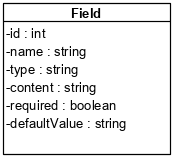
\includegraphics[width=0.25\textwidth]{figures/Classes/FieldAttributes.png}
    \caption{Field class}
    \label{fig:FieldClass}
\end{figure}